\subsection{Digit 0, 1, 2, 3}
\label{sec:IND_CHECK}

Once the 4 digit password is entered with the keypad, the system has to compare it with the password preset by the user with the dip-switches.

\medskip

In order to do this, each of the 4 digits of the password is compared by a different GAL due to a limitation in the number of input pins. This example corresponds to the DIGIT\_0 of the password, but the other three work in the same way, thus, only one of them is explained. 

\medskip

For the GAL to know which of the digits is the first one, the Address (A) from the memory device is read. In this case, if the Address is $00$, we have the digit required at the Data Bus (D).\medskip

We will now go over the different states of the Finite State Machine: \medskip

\medskip
\textit{\bm{$Q_0$}}
\medskip

By default, the Output of the GAL, \textit{DIGIT\_0} is at a LOW state. The GAL checks 4 inputs, namely \textit{DONE}, the predefined password (via the dip switch) \textit{PASS0}, the address value, \textit{A} and the value stored in the RAM at that specific address, \textit{D}. If the \textit{DONE} pin is ON, meaning that the whole password has been introduced, the address is "00" (for this particular digit), and \textit{PASS0} = \textit{D}, then the state is changed and the FSM moves to \textit{Q1}.\medskip

\textit{\bm{$Q_1$}}
\medskip

In this state, the GAL device will output a HIGH at \textit{DIGIT\_0} indicating that the first digit of the password is correct. \medskip

Finally, when the \textit{RESET} signal is detected, the state switches back to Q0 and the \textit{DIGIT\_0} pin is pulled LOW, effectively resetting the FSM. \medskip

To illustrate the different states and the transitions between them we have included the following diagram:

\begin{figure}[H]
    \centering
    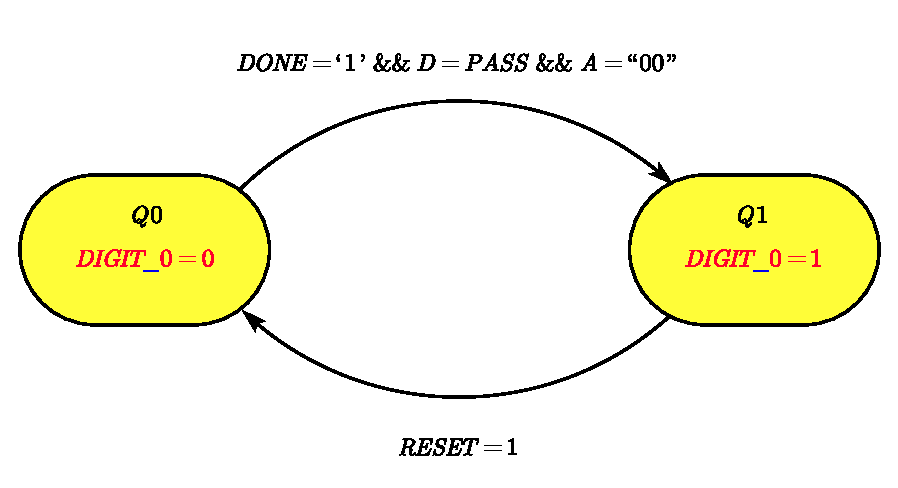
\includegraphics[scale = 0.6]{Graphics/DIGITS/DIGITS_FSM.pdf}
    \caption{Digits [0...3] FSM}
    \label{fig:DIGITS_FSM}
\end{figure}


\clearpage

The VHDL code describing this subsystem is attached below:

\inputcode{Code/DIGITS.vhd}

\clearpage

The Proteus subassembly corresponding to the 4 digits can be seen below:

\begin{figure}[H]
    \centering
    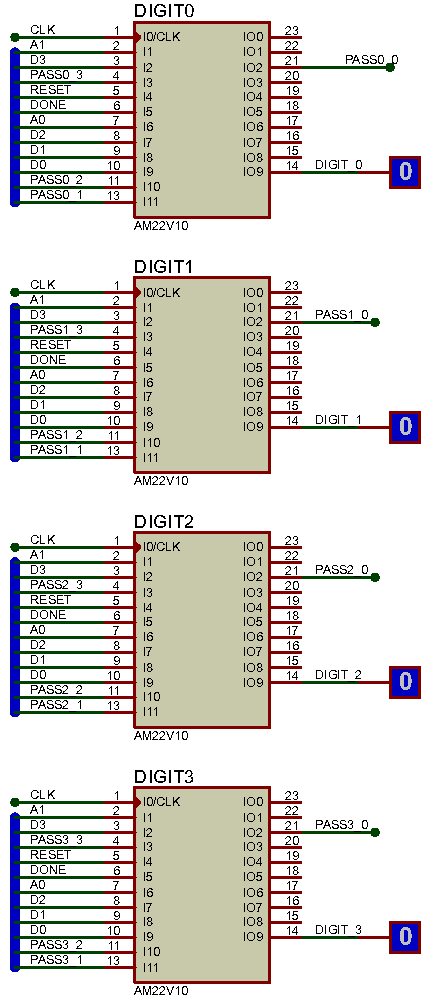
\includegraphics[scale = 1]{Graphics/DIGITS/DIGITS_PROTEUS.PDF}
    \caption{Proteus Subassembly of Digits [0...3]}
    \label{fig:DIGITS_PROTEUS}
\end{figure}


